\documentclass[review]{elsarticle}

\usepackage[]{geometry}
\usepackage{amsmath}
\usepackage{amssymb}
\usepackage{graphicx}
\usepackage{xcolor}
\usepackage{hyperref}
\usepackage{natbib}
\bibliographystyle{elsarticle-harv}
\biboptions{authoryear}

\newcommand{\ra}{\rightarrow}
\newcommand{\afs}[2]{\Phi_{#1}^{(#2)}}
\newcommand{\Dfrac}[2]{%
  \ooalign{%
    $\genfrac{}{}{1.2pt}0{#1}{#2}$\cr%
    $\color{white}\genfrac{}{}{.4pt}0{\phantom{#1}}{\phantom{#2}}$}%
}
\newcommand{\cond}{\middle\vert}
\newcommand{\dslash}{/\!\!/}
\newcommand{\Coalc}[4]{\begin{bmatrix}#1\dslash #2 \\ #3\dslash #4 \end{bmatrix}}

\newcommand{\sgcomment}[1]{{\color{red}{SG: #1}}}
\newcommand{\ikcomment}[1]{{\color{blue}{IK: #1}}}
\newcommand{\Var}{\operatorname{Var}}
\journal{Theoretical Population Biology}

\begin{document}
\begin{frontmatter}
  \title{ Taming strong selection with large sample sizes. }

  \author{Ivan Krukov}
  \author{Simon Gravel}

  \begin{abstract}
    The fate of mutations and the genetic load of populations depend on the relative importance of
    genetic drift and natural selection. In addition, the accuracy of numerical models of evolution
    depends on the strength of both selection and drift: strong selection breaks the assumptions of
    the nearly neutral model, and strong drift coupled with large sample sizes breaks the
    Kingman's coalescent model.
  
    Thus, the regime with strong selection and large sample sizes appears particularly daunting.
    However, we find that the competition between drift and natural selection in this regime can be
    used to define asymptotically closed recursions for the distribution of allele
    frequencies -- well beyond the strong selection limit.
 
    We construct the relevant transition matrices, show how they can be used to accurately compute
    distributions of allele frequencies, and discuss the boundaries of this analytically tractable
    regime.
  
    Selection becomes more analytically tractable when the sample size $n$ is larger than twice the
    population-scaled selection coefficient: $n \ge 2Ns$ ($4Ns$ in diploids). In this regime, the
    expected number of coalescent events is larger than the number of selective events. We also
    derive the exact distribution of the number of sampled lineages, and offer a Gaussian
    approximation for a more tractable solution.
  \end{abstract}

\end{frontmatter}

\section{Introduction}
\label{sec:introduciton}

The allele frequency spectrum (\textit{AFS}) is an important summary of genetic diversity that is
commonly used to infer demographic history and natural selection (\textit{e.g.}
\cite{GutenkunstEtAl2009, KammEtAl2017, JouganousEtAl2017}). Given a demographic scenario of
population size histories and migrations, the diffusion approximation or coalescent simulations can
be used to obtain a predicted \textit{AFS}. By comparing predictions to the observed \textit{AFS},
one can compute likelihoods for different demographic scenarios. Unfortunately, the \textit{AFS}
calculations can be time consuming under complex demographic models, for example with multiple
populations, or with large sample sizes.

In the absence of selection, efficient computational shortcuts can be used. Coalescence models such
as \citep{fastsimcoal2, KammEtAl2017} can efficiently compute the \textit{AFS} or subsets of it. In
addition, recursion equations have been derived for moments of the neutral allele frequency
distribution \citep{KimuraCrow1964,Ewens1972,JouganousEtAl2017}. Recently, these recursions have
been useful in fitting complex demographic models to genetic data
\citep{JouganousEtAl2017,KammEtAl2017}.
 
In the presence of natural selection, coalescent models become much more complicated, and the
corresponding recursion equations do not close but
form a very large or infinite set of coupled equations \citep{DonnellyKurtz1999, JouganousEtAl2017}. Moment-based closure approximations
have been developed \citep{JouganousEtAl2017}, but these are not robust to strong selection and
their convergence properties are not well understood.

Closure of the moment equations under the neutral Wright-Fisher model occurs because the number $n_p$ of
distinct parental lineages that are sampled when drawing $n_o$ offspring lineages is at most $n_o$, and can be less if common ancestors are found (i.e., if there are coalescent events): 
$n_p \le n_o$ (see Table \ref{tab:symbols} for the notation used). This does not
hold under negative selection -- selective deaths can require the drawing of $n_p>n_o$  \citep{DonnellyKurtz1999a,
  JouganousEtAl2017}. This possible increase is made explicit, for example, in the framework of the ancestral
selection graph \citep{KroneNeuhauser1997}.

The number of relevant lineages as we go back in time is a random variable that depends on the relative
importance of drift (controlled by the population size $N$) and selection (controlled by the selection coefficient $s$), but also on the sample size $n_o$. 
The number of in-sample coalescent events per generation scales as the square of the sample size $n_o$,
while the number of selective deaths is linear in $n_o$. For sufficiently large
samples, the expected number of selective deaths will be smaller than common ancestry events, which would prevent the
increase in the number of lineages. If we can show that this holds not just in expectation, but almost always,  
we can obtain recursion equations that are almost closed. 
 
Large sample sizes also bring in the complication of simultaneous coalescent events
\citep{BhaskarEtAl2014}. The additional combinatorial possibilities make the computation 
of transition matrices for recursion equations more difficult. 
In this article we derive these transition matrices, and
show that these are asymptotically closed even under strong selection. %In fact, the multi-way
%coalescent events deplete the number of lineages faster than pairwise events further counter-acting
%the selection effects. 
We show that these transition matrices can be used to accurately model the 
distribution of allele frequencies in moderate to large samples and strong selection.

In short, modeling large sample sizes makes it easier to accurately account for strong selection. 


\section{Methods}
\label{sec:methods}

We consider a haploid Wright-Fisher model with $N$ individuals per generation, focusing on a single
biallelic locus. For a present-day sample with $n_o$ offspring lineages at time $t$, we will be
looking for recursion equations for the allele frequency spectrum, $\afs{n_o}{t}(i_o)$, which we
define as the probability of observing $i_o$ copies of the derived allele in a sample of size $n_o$.
We will do so by considering the process of drawing parental alleles (at time $t-1$) for this finite
sample.
\begin{table}
  \centering
  \begin{tabular}{l|p{100mm}}
    Symbol & Meaning\\
    \hline
    $N$ & Population size\\
    $n_p$ & Number of sampled parental lineages (actual plus rejected samples due to selective deaths)\\
    $n_g$ & Number of gametes (intermediate)\\
    $n_o$ & Number of offspring, sample size\\
    $i_p$ & Number of derived alleles in parents\\
    $i_o$ & Number of derived alleles in offspring\\
    $t$ & Time, in generations\\
    $\Phi_{n_o}^{t}(i_o)$ & Allele frequency spectrum in $n_o$ at generation $t$\\
    $s$ & Selection advantage of the derived allele\\
    $r$ & Number of selection events (rejections) in the sample\\
    $x_p$ & Frequency of derived allele in parental generation\\
    $i_o \dslash n_o$ & A sample with $i_o$ derived alleles ``out of'' $n_o$ total lineages\\
    $\mathbf{H}\Coalc{i_p}{n_p}{i_o}{n_o}$ & Hypergeometric probability -
                                             sample $i_o \dslash n_o$ in offspring from $i_p \dslash n_p$ in parental generation\\
    $\mathbf{T}_{r}\Coalc{i_p}{n_p}{i_o}{n_o}$ & Probability of transition from $i_p \dslash n_p$ in parents
                                                 to $i_o \dslash n_o$ in offspring, with $r$ selective events -
                                                 see text for a more detailed description\\
  \end{tabular}
  \caption{\label{tab:symbols} Table of symbols}
\end{table}
%Under neutral evolution, each offspring picks a lineage at random with replacement, and the number
%$n_p$ of distinct parental lineages is smaller than $n_o$ (Fig.\ref{fig:schematic}A).

To model selection as part of our sampling process, we consider that a parental lineage carrying a
derived allele can be `rejected' as a result of selective death with probability $s\ge0$ (Fig.
\ref{fig:schematic}B, broken line). In such case, we keep sampling until a successful draw. This is
equivalent to the usual formulation of the Wright-Fisher model: the probability of drawing a copy of the
derived allele is $1-s$ times the probability of drawing a copy of the ancestral allele. And, because the drawing
process depends on the parental allele of both successful and rejected draws, the \textit{AFS} in the
offspring will depend on the state of the $n_p$ distinct parental lineages that were sampled. 
Because of selective rejection, $n_p$ can be larger than
$n_o$. %When referring to sampled lineages ($n_p$), we mean any lineages that have been sampled and
%possibly rejected.

To disentangle the effects of drift and selection, we may also make explicit the number of gametes
sampled in the process, $n_g$ (Fig. \ref{fig:schematic}C). The difference $n_g-n_o  \ge 0$
depends only on the number of selective deaths, whereas the difference $n_p-n_g \le 0$ depends
only on the number of coalescence events. We will use this notation with $n_g$ in section
\ref{sec:asympt}. %Note that in Figure \ref{fig:schematic}A,B, the gametes are implicit.

\begin{figure}[h]
  \centering
  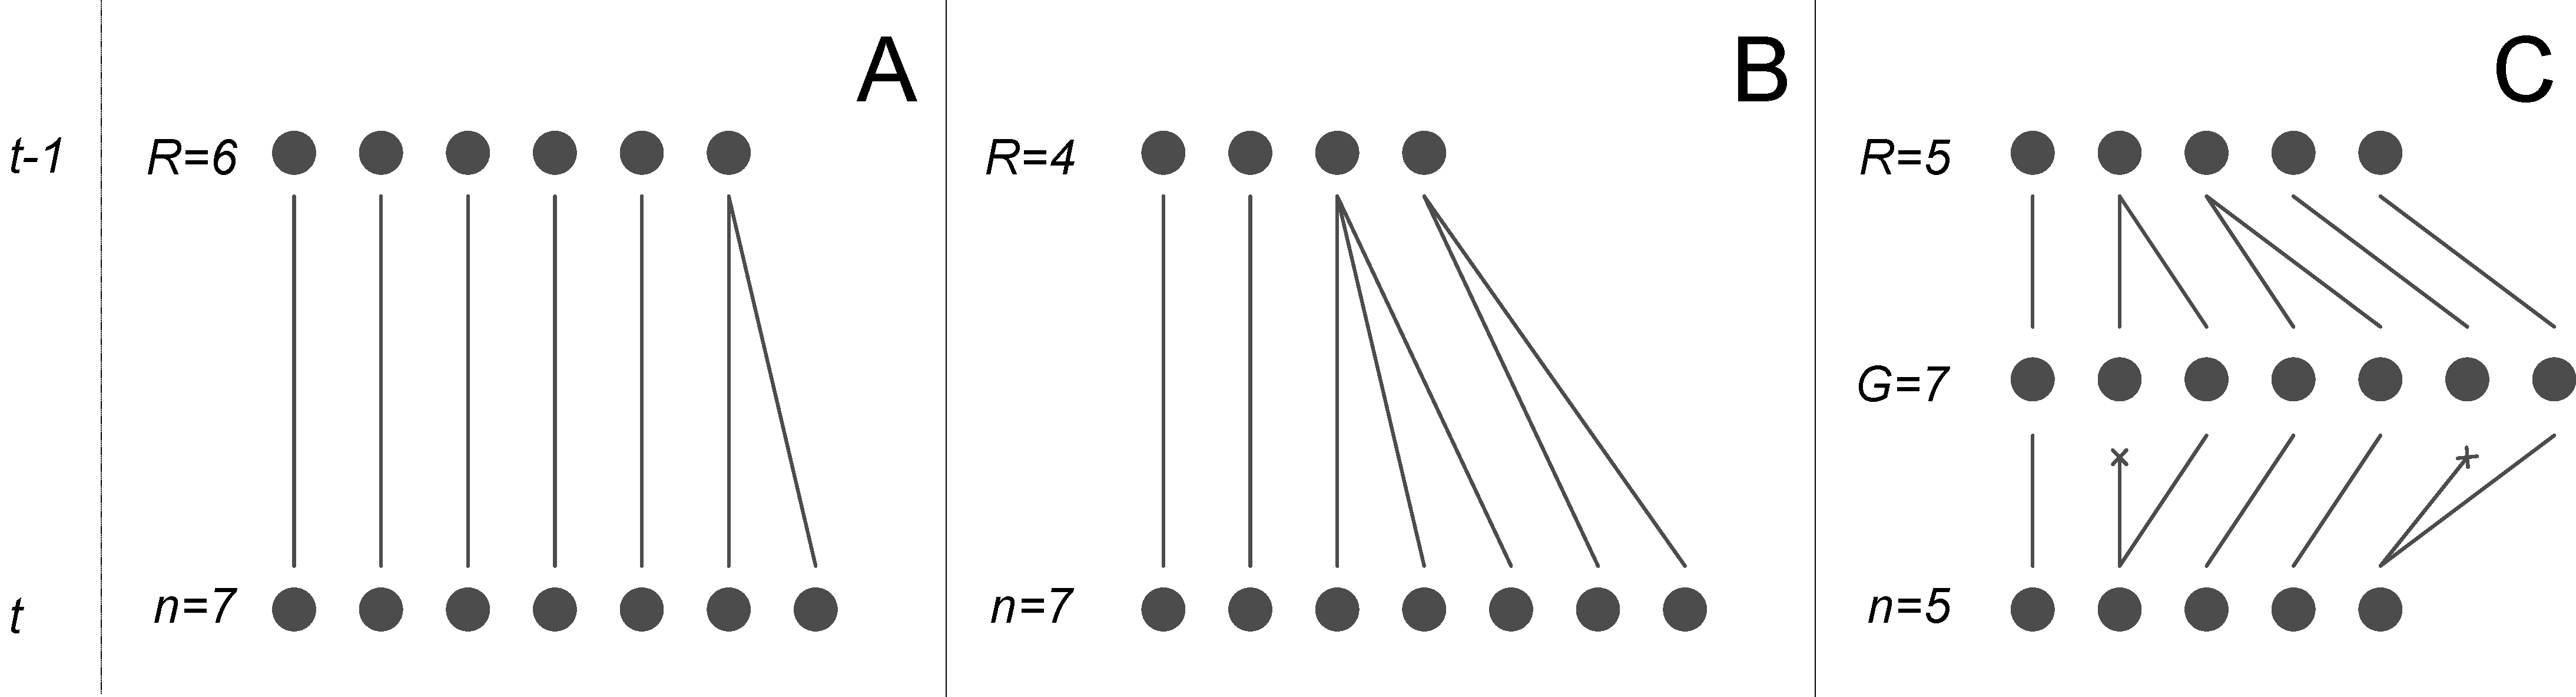
\includegraphics[width=1.0\textwidth]{fig/schematic.pdf}
  \caption{\label{fig:schematic} Realizations of sampling parental lineages under neutrality (A) and
    under selection (B,C). The top and bottom rows respectively represent the $n_p$ parents and
    $n_o$ offspring, with the middle row in panel (C) representing the $n_g$ gametes. Filled circles
    indicate the $i_p$, $i_g$, or $i_o$ copies of the derived allele. A line connecting two circles
    represents a successful draw, a broken line - a selective death triggering a redraw. }
\end{figure}

To express the allele-frequency spectrum $\afs{n_o}{t}(i_o)$ for $n_o$ offspring in terms of the parental
\textit{AFS} at $t-1$, we can sum over random variables $n_p$ and the number $i_p$ of distinct derived alleles
among the parents:

\begin{equation}
  \afs{n_o}{t}(i_o)=P_{n_o} (i_o) =\sum_{n_p,i_p} P_{n_o}(i_o,i_p,n_p),
\end{equation}
where the subscript $n_o$ indicates dependence on parameter $n_o$. To obtain a recursion on the
\textit{AFS}, we use an exchangeability property of the parental lineages: the order
 in which we draw previously unsampled parental lineages in the Wright-Fisher
model is random. 
In other words, we could draw a random permutation of the parental population, and
select parents in order from this permutation. We will separate properties of this permutation,
which depend only on parental \textit{AFS}, from properties of Wright-Fisher sampling, which depend on population size and selection coefficients.
 Concretely, the event $(i_p,n_p)$ that we draw exactly $i_p$ derived alleles and $n_p$ distinct parents can be expressed as the intersection of two events, $\mathcal{C}(i_p,n_p)$
and $\mathcal{S}_{n_p}$. Event $\mathcal{C}(i_p,n_p)$ specifies that the first $n_p$ parental
lineages from the random permutation carry $i_p$ derived alleles. Event $\mathcal{S}_{n_p}$
requires that the Wright-Fisher drawing process \textit{stops} after exactly $n_p$ parental lineages
have been drawn. Event $\mathcal{C}(i_p, n_p)$ is a property of the allele frequency distribution 
in the parental generation: $P(\mathcal{C}_{n_p}(i_p)) =\afs{n_p}{t} (i_p)$ by definition of the \textit{AFS}. Thus 

\begin{equation}
  \begin{split}
    \afs{n_o}{t}(i_o)&= \sum_{n_p,i_p} P_{n_o}(i_o, \mathcal{S}_{n_p}, \mathcal{C}(i_p,n_p) )\\
    &=   \sum_{n_p,i_p} P_{n_o}(i_o, \mathcal{S}_{n_p}| \mathcal{C}(i_p,n_p) ) P(\mathcal{C}(i_p,n_p))\\
    &=   \sum_{n_p,i_p} P_{n_o}(i_o, \mathcal{S}_{n_p}| \mathcal{C}(i_p,n_p) )  \afs{n_p}{t-1}(i_p)\\
    &\equiv  \sum_{n_p,i_p}  \mathbf{T}_{n_p,n_o}     \afs{n_p}{t-1}(i_p).
  \end{split}
  \label{eq:recur}
\end{equation}
where the $\mathbf{T}_{n_p,n_o}$ can be thought of as $(n_o+1) \times (n_p+1)$ transition
probability matrix, whose row and column indices correspond to the number of derived alleles in the
offspring and contributing parental lineages, respectively.

The AFS  $\afs{n_p}{t-1}(i_p)$ for any  $n_p\leq n_o$ can be obtained by downsampling from $\afs{n_o}{t-1}$ (\textit{i.e.}, $\afs{n_p}{t-1} =
\mathbf{H}_{n_p,n_o} \afs{n_o}{t-1}$ for hypergeometric projection matrix $\mathbf{H}_{n_p,n_o}$ if
$n_p\leq n_o$), so Equation \eqref{eq:recur} provides a closed form recursion for $\Phi_{n_o}$ under neutrality.
This property was used in \cite{JouganousEtAl2017} to efficiently compute distributions of allele
frequencies under neutrality and in small sample sizes.

Under selection, $n_{p}$ may be larger than $n_o$, leading to a set of $N$ coupled equations that is
typically too large to solve numerically (in the diffusion limit, the number of coupled equations is
infinite). But if the number of drift events is typically larger than the number of selective
deaths, as happens in large sample sizes, the coupling is weak and we can restore approximate
closure by truncating the summation in Eq. \ref{eq:recur}:

\begin{equation}
\begin{split}
  \afs{n_o}{t}(i_o)
  &\simeq \sum_{n_p=1}^{n_{o}} \mathbf{T}_{n_p,n_o}                      \afs{n_p}{t-1}\\
  &=      \sum_{n_p=1}^{n_{o}} \mathbf{T}_{n_p,n_o} \mathbf{H}_{n_p,n_o} \afs{n_o}{t-1}\\
  &\equiv \mathbf{Q}_{n_o}                                               \afs{n_o}{t-1}\\
\end{split}
\label{eq:truncated}
\end{equation}

A jackknife approximation \citep{Gravel2016} can be used to simulate the drawing of a small number
of additional lineages and improve upon this closure approximation
($\afs{n_p}{t} \simeq J_{n_p,n_o} \afs{n_o}{t}$ with $n_p>n_o$). \cite{JouganousEtAl2017} used the
jackknife to derive approximate recursion equations under weak selection. We will show below that
closure is asymptotically maintained for large sample sizes even without requiring a jackknife
approximation.

Our first goal is to obtain an explicit recursion for the matrices in \eqref{eq:recur}. To do so, we
will need to account for multiple coalescent events, which will require some careful bookkeeping.

\section{Transition probability matrices}
\label{sec:trans-mat}

\subsection{Constructing the transition matrix}
\label{subsec:trans-mat}

Even though $\mathbf{T}_{n_p,n_o}$ in Eq. \ref{eq:recur} is a combinatorial probability
describing a single generation in the Wright-Fisher model, we were unable to compute an analytical
expression for it, while allowing for multiple coalescences and multiple selective events. 
However,
we can obtain fairly simple recursions by noting that properties of a sample of size $n_o$ are
related to properties of samples of size $n_o-1.$ Similar recursions on sample size were used for
describing large sample size effects without selection in \citep{BhaskarEtAl2014}. In this section,
we provide some mathematical intuition for the recursion equation, and a more detailed derivation is provided in
Appendix \ref{subsec:apx:tpm}.

We can think of Wright-Fisher sampling as being performed one offspring at a time,
and even one draw at a time. We will define recursions by conditioning on the last draw, 
whether it is successful or failed. 
To keep track of the number $r$ of unsuccessful draws for the current offspring, we define $\mathbf{T}_{r}\Coalc{i_p}{n_p}{i_o}{n_o}$ as the probability
$P_{n_o}(\mathbf{Q}(i_o,r) | i_p, n_p)$ of the event $\mathbf{Q}(i_o,r)$ that exactly $i_o$ of the
first $n_o$ successfully drawn offspring are derived, and that the following $r$ draws are selective
deaths - Figure \ref{fig:rec-selection-dynamic-fail}. This bracket notation is convenient to keep track of
the number of relevant parental lineages (at the top) and offspring lineages (at the bottom), at the
cost of obscuring their different probabilistic role.

The recursion can be broken down in a recursion over $r$, determined by failed draws, 
and a recursion over $n_o$, determined by successful draws.  
The recursion over $r$ is shown at the bottom of
Figure \ref{fig:rec-selection-dynamic-fail} (cases \textit{rC,rD}). If the last draw was rejected, the sampling 
prior to the last draw must have ended with $r-1$ rejected draws. We
must simply track whether the last rejected draw was from a previously drawn parental lineage (case
\textit{rD}), in which case the number of parental lineages is unchanged, or of a new lineage (case
\textit{rC}), in which case the sample with $r-1$ rejections must have had exactly one fewer distinct parent and 
one fewer derived parental allele than the full sample.  
 
Thus we can obtain $\mathbf{T}_{r}\Coalc{i_p}{n_p}{i_o}{n_o}$ from
$\mathbf{T}_{r-1}\Coalc{i_p-1}{n_p-1}{i_o}{n_o}$ and $\mathbf{T}_{r-1}\Coalc{i_p}{n_p}{i_o}{n_o},$
and recursively back to terms of the form $\mathbf{T}_{0}\Coalc{i_p'}{n_p'}{i_o}{n_o}$, with $n_p'\leq n_p$
  
To progress further and express $\mathbf{T}_{0}\Coalc{\cdot}{\cdot}{i_o}{n_o}$ in terms of
$\mathbf{T}_{r}\Coalc{\cdot}{\cdot}{\cdot}{n_o-1}$, we condition on the last
successful draw. This last successful draw can be a previously sampled parental lineage (cases B,D on Figure \ref{fig:rec-selection-dynamic-fail}), or
unsampled (cases A,C); and can be derived (cases A,B), or ancestral (cases C,D), giving rise to four cases.
  
A challenge with this recursion is that the number of rejected lineages $r$ for each individual draws 
can be infinite.
 However, the probability of having multiple selective deaths for a single successful draw decreases,
rapidly, as $s^r.$ We therefore modify the Wright-Fisher model such that at most $r_{max}$ failed
draws \emph{per offpsring lineage} are allowed, after which the next draw is immune to selection. Given
$s<1$, we can easily pick $r_{max}$ to ensure excellent convergence. For example, with $s=0.01$, 
which corresponds to $Ns=100$ with $N=10 000$, the probability of having more than 
four selective deaths is less than $10^{-10}$, and the probability of having more than 8 selective deaths is 
less than $10^{-20}.$ We have used $r_{max}=4$ in numerical calculations presented below. 

  
Using these two recursions, and using caching to avoid re-computing previously computed values,
we can systematically compute all the terms in Equation \ref{fig:rec-selection-dynamic-fail}.




\begin{figure}
  \centering
  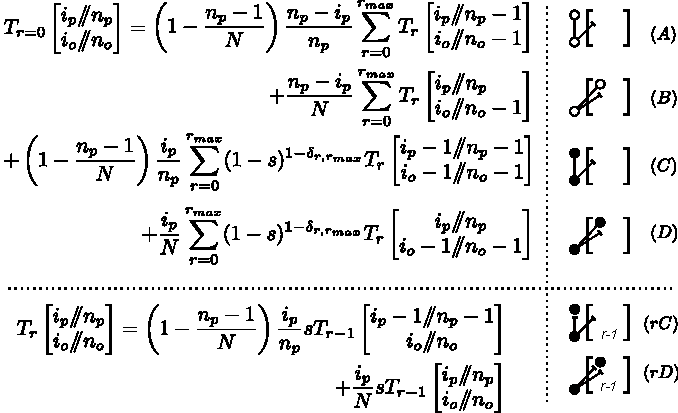
\includegraphics[width=0.9\textwidth]{fig/recurrence-selection-dynamic-failures-annotated.pdf}

  \caption{Recursion construct for transition probability with selection, accounting for multiple
    kinds of coalescent events. The right hand panel represents summands on the left graphically.
    Filled and empty circles represent derived and ancestral alleles. Solid and broken lines are
    successful lineage draws and re-draws due to selection. Double lines represent potentially
    multiple draws. Square brackets represent events in a smaller sample size ($n_o-1$). Summands
    (\textit{A-D}) are successful draws where the last lineage is ancestral (\textit{A,B}) or
    derived (\textit{C,D}). Note that these terms depend on the probability that there were between
    $0$ to $r_{max}$ selective events in sample size $n_o-1$. Terms \textit{rC} and \textit{rD}
    represent the probability that last selection re-draw was due to a lineage from outside
    (\textit{rC}) or within (\textit{rD}) the sample. See table \ref{tab:symbols} for notation used.
  }

  \label{fig:rec-selection-dynamic-fail}
\end{figure}
 
The set of selection transition probability matrices $\mathbf{T}$ requires $O(r_{max}n_o^2 n_p^2)$
operations to construct: Since each term $\mathbf{T}_{r}$ (with $r>0$)  in the recursion requires a constant number of operations, 
the computational complexity depends on the number of terms we need to calculate. We will need to compute terms of the form 
 $\mathbf{T}_{r}\Coalc{i_p'}{n_p'}{i_o'}{n_o'}$, with $1 \leq n_o'<n_o$, $i_o' \leq n_o'$, $0\leq i_p' \leq n_p' \leq n_p$, and $0\leq n_p' \leq \alpha n_o$, 
 and $0\leq r \leq r_{max},$ leading to the bound $O(r_{max}n_o^2 n_p^2).$   
 
 
 
 The terms  $\mathbf{T}_{0}$ have a bound of the same form (i.e., there are at most $O(n_o^2 n_p^2)$ terms, each requiring $r_{max}$ computations).  
Finally, the truncated matrix $\mathbf{Q}_{n_o} = \sum_{n_p=1}^{n_{o}} \mathbf{T}_{n_p,n_o} \mathbf{H}_{n_p,n_o}$ can be constructed in $O(n_o^4)$.
\sgcomment{I think some of these $n_o$ might be $n_p$'s}

This is moderately more complex than in the neutral case, where recursions can be computed in $O(n^3)$ as in \cite{BhaskarEtAl2014}.

\subsection{Calculation of allele frequency spectra}
\label{subsec:afs}

Once the truncated matrix
$\mathbf{Q}_{n_o} = \sum_{n_p=1}^{n_{o}} \mathbf{T}_{n_p,n_o} \mathbf{H}_{n_p,n_o}$
\eqref{eq:truncated} is constructed, it can be used to calculate the allele frequency spectrum. To
validate the method, we first use the equilibrium distribution where exact solutions are available
\citep{Krukov2016}. In the infinite sites model at equilibrium, we can compute the
equilibrium \textit{AFS} $\Phi$ in a finite sample as a solution to a linear system:

\begin{equation}
  \label{eq:sfs-calc}
  \Phi = \mathbf{Q}\Phi  + n \mu e_1
\end{equation}
where $\mu$ is the per-site (forward) mutation rate, and $e_1$ is the first column of the identity
matrix of size $n$. Figure \ref{fig:strong-selection} shows the comparison of the \textit{AFS}
calculated from Equation \eqref{eq:sfs-calc}, the diffusion approximation
\cite[eq. 9.23]{Ewens2004}, and the calculation performed in \texttt{Moments}
\citep{JouganousEtAl2017}.

Figures \ref{fig:strong-selection}A-C show that there is a disagreement between the exact
Wright-Fisher and the diffusion solutions for singletons and doubletons. This effect increases as in
large sample sizes, as $n \ra N$, and has been reported by \citep{BhaskarEtAl2014}. There is a also
a divergence at high frequency of the derived allele. %The Wright-Fisher and the present model are
%both absorbing at fixation of the derived allele, while the diffusion models are not. 

Figure \ref{fig:strong-selection}D-F shows a comparison at strong negative $Ns=50$, with a
sample size of $100$ and population sizes ranging from $N=100$ to  $N=1000.$  
The recursions presented here provide excellent agreement with the exact result even 
where the diffusion-based approaches fail. 

When the sample is the entire population, as in panel F, the present method is not needed since
exact recursion equations can be obtained from the binomial distribution 
(i.e., there is no computational benefit to consider a subsample that is as large as the entire population). 
The present approach will be useful if exact recursions can be obtained for sample sizes that are appreciably smaller
than $N$. We therefore seek asymptotic results for the convergence of the recursion approach.



\begin{figure}
  \centering
  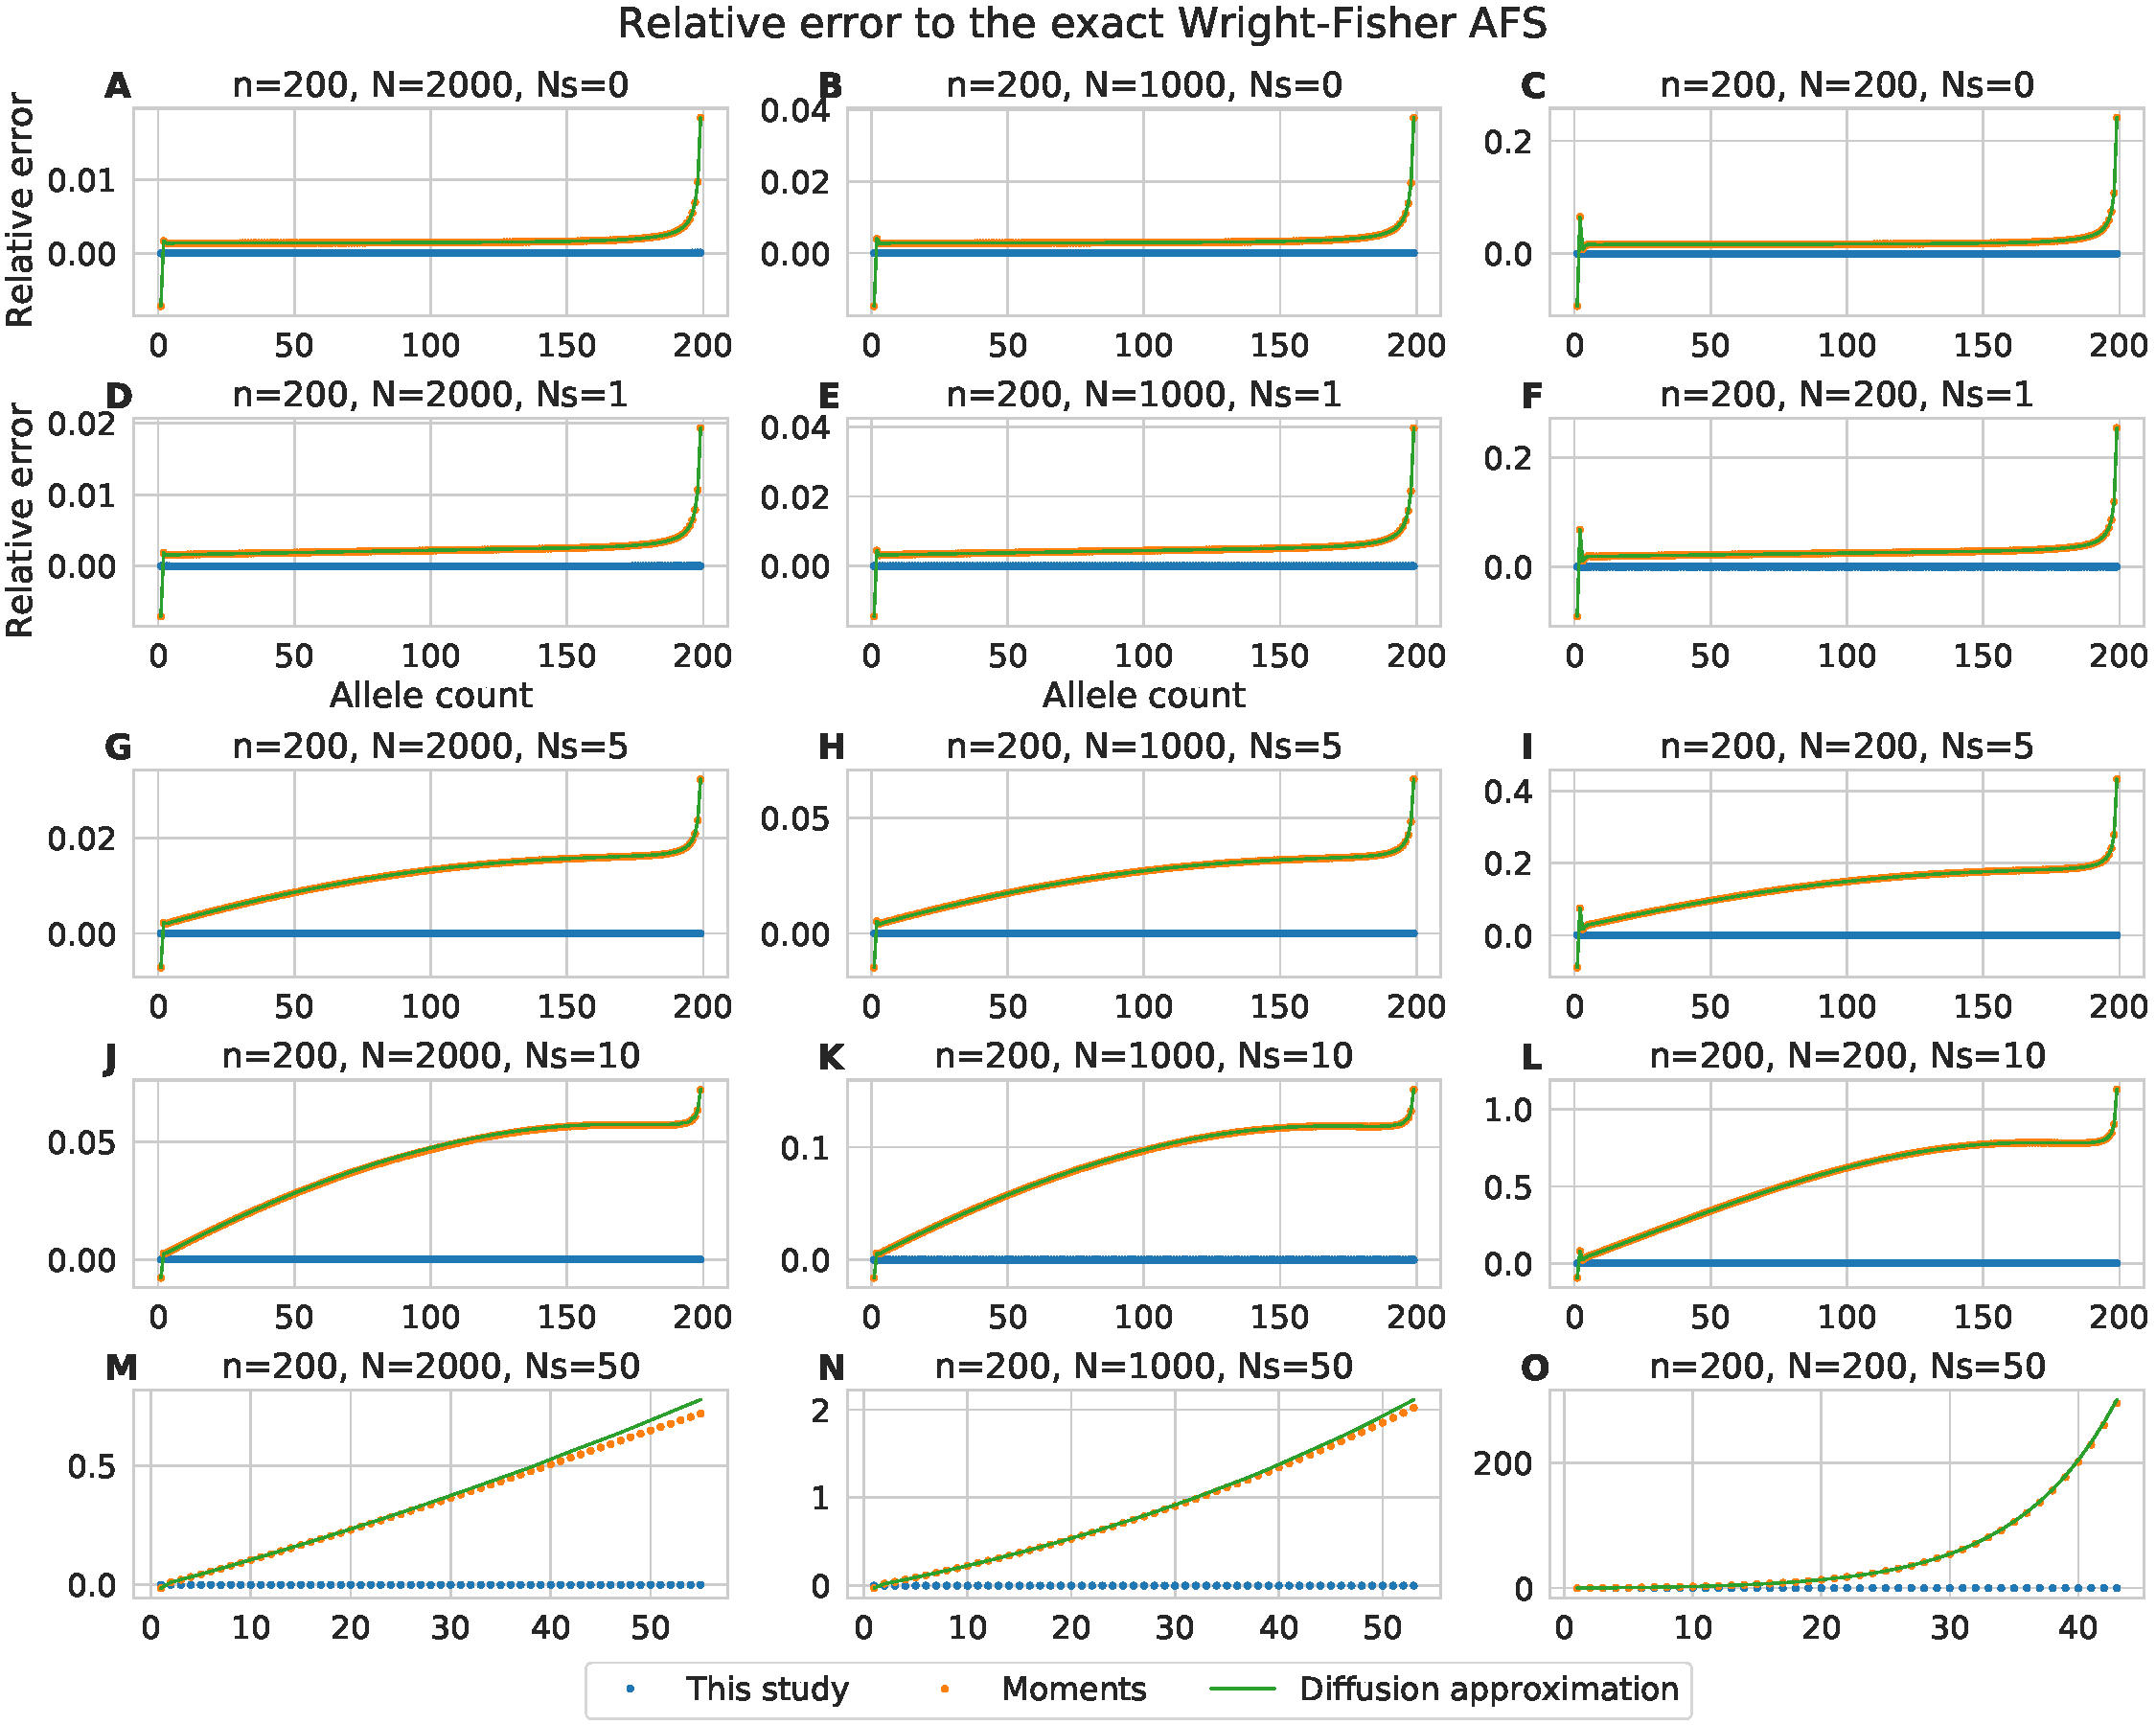
\includegraphics[width=0.7\textheight]{fig/strong_selection_six_panel.pdf}
  \caption{Normalized allele frequency spectra in a sample of size $n=100$, for neutral (Ns=0)
    (A,B,C), or highly deleterious alleles ($Ns=50$) (D,E,F). (A) shows the frequency spectrum in a
    sample from a large population ($N=1000$), (B) intermediate ($N=500$), and (C) small population
    ($N=100$). (D,E,F) same, for deleterious allele. The Y-axes are at different scales between the
    panels, to better indicate disagreement. The X-axes for panels (D,E,F) were truncated
    when the \textit{AFS} probability dropped below $10^{-12}$. }
  \label{fig:strong-selection}
\end{figure}

\subsection{Missing probability}
\label{subsec:missing}

Truncation in equation \ref{eq:truncated} means that if $n_p > n_o$, some probability will be lost. 
\sgcomment{Did you do re-normalization of the truncated matrix?} 

%The transition matrix $\mathbf{Q}_{n_o}(i_p, i_o),$ in equation
%\eqref{eq:truncated}, also has a probabilistic meaning:

The $(i_p,i_o)^\text{th}$ element of matrix $Q_{n_o}$ is the probability
$P_{n_o}(i_o, \mathcal{S'}_{n_o}| \mathcal{C'}(i_p,n_p))$ that we observe $i_o$ derived alleles in
a sample of size $n_o$ and that we draw \emph{at most} $n_o$ distinct parental lineages (event
$\mathcal{S'}_{n_o}$), given event $\mathcal{C'}(i_p,n_p)$ that $i_p$ of the first
$n_p$ parental alleles are derived.

By summing $\sum_{i_o} \mathbf{Q}_{n_o}(i_p, i_o),$ we therefore get the proportion of draws that
were not truncated. $1-\sum_{i_o} \mathbf{Q}_{n_o}(i_p, i_o)$ is therefore the fraction of
unaccounted-for draws due to truncation, given $i_p$ derived among the first $n_o$ parental
alleles. Since only derived lineages experience selection, the largest number of resampling events,
and therefore the largest number of unaccounted lineages, occurs when all alleles are derived,
$i_o = n_o$.

Figure \ref{fig:apx:missing} shows this probability under this worst-case scenario. The probability
of missing lineages first increases with increasing sample size, as the number of draws that can
result in selective deaths increases. However, the number of drift events eventually overtakes the
number of selective events, and the probability that we need additional lineages decreases rapidly
with sample sizes. With large enough sample sizes, the missing probability can be made very small.

\subsection{Distribution of number of sampled lineages}
\label{subsec:distribution}

To get an analytical expression for the probability of missing lineages,
we consider the probability that $n_p$ parents have been sampled,
\begin{align}
  \label{eq:conditional}
  P(n_p | n_o) = \sum_{n_g} P(n_p | n_g,n_o)P(n_g | n_o) = \sum_{n_g} P(n_p | n_g)P(n_g | n_o) 
\end{align}
where $n_p$ and $n_g$ is the number of sampled parents and gametes, respectively (Fig.
\ref{fig:schematic}C). 

The distribution over the number of gametes, $n_g$, is given by the negative binomial,
parameterized by the number of successes $n_o$, and the probability of a successful draw is $1-x_ps$, where $x_p$ is
the derived allele frequency in the parental population,
\begin{align}
  \label{eq:neg-binomial-trials}
  P(n_g|n_o) = \binom{n_g-1}{n_o-1}(1-x_ps)^{n_o}(x_ps)^{n_g-n_o},
\end{align}
where $x_p$ is the proportion of derived alleles in the parental generation.

Given $n_g$, the number of parental lineages $n_p$ follows the modified occupancy (also known as
Arfwedson) distribution \citep{Wakeley2009,ONeill2019,JohnsonEtAl2005}:

\begin{align}
  \label{eq:occupancy}
  P(n_p|n_g) = \frac{S_2(n_g,n_p) N!}{(N-n_p)! N^{n_g}}
\end{align}
where $S_2(n_g,n_p)$ is a Stirling number of the second kind, which is the number of ways to
partition $n_g$ gametes into $n_p$ parents (see \cite{JohnsonEtAl2005} section 10.4 for a thorough
treatment).

Combining the two distributions together through Eq. \ref{eq:conditional}, we get:

\begin{align}
  \label{eq:lineages-in-past}
   P(n_p|n_o) = \sum_{n_g=1}^{\infty} \frac{S_2(n_g,n_p) N!}{(N-n_p)! N^{n_g}} \binom{n_g-1}{n_o-1}(1-x_ps)^{n_o}(x_ps)^{n_g-n_o}
\end{align}

We did not find an analytical expresion for this sum, but it can be computed
efficiently using methods presented in \citep{ONeill2019}. Figure \ref{fig:combined}A (dots) shows
the distribution of the number of contributing parental lineages for several selection coefficients with $n_o=200$ 
and $x_p=1$. %In the absence of selection (not shown), the distribution has
%zero probability above $n_o=200$, as no extra lineages can be sampled. 
As the strength of selection
is increased, we begin requiring larger numbers of lineages, while with increasing sample size,
there is a decrease in required lineages due to coalescent events.

\begin{figure}
  \centering
  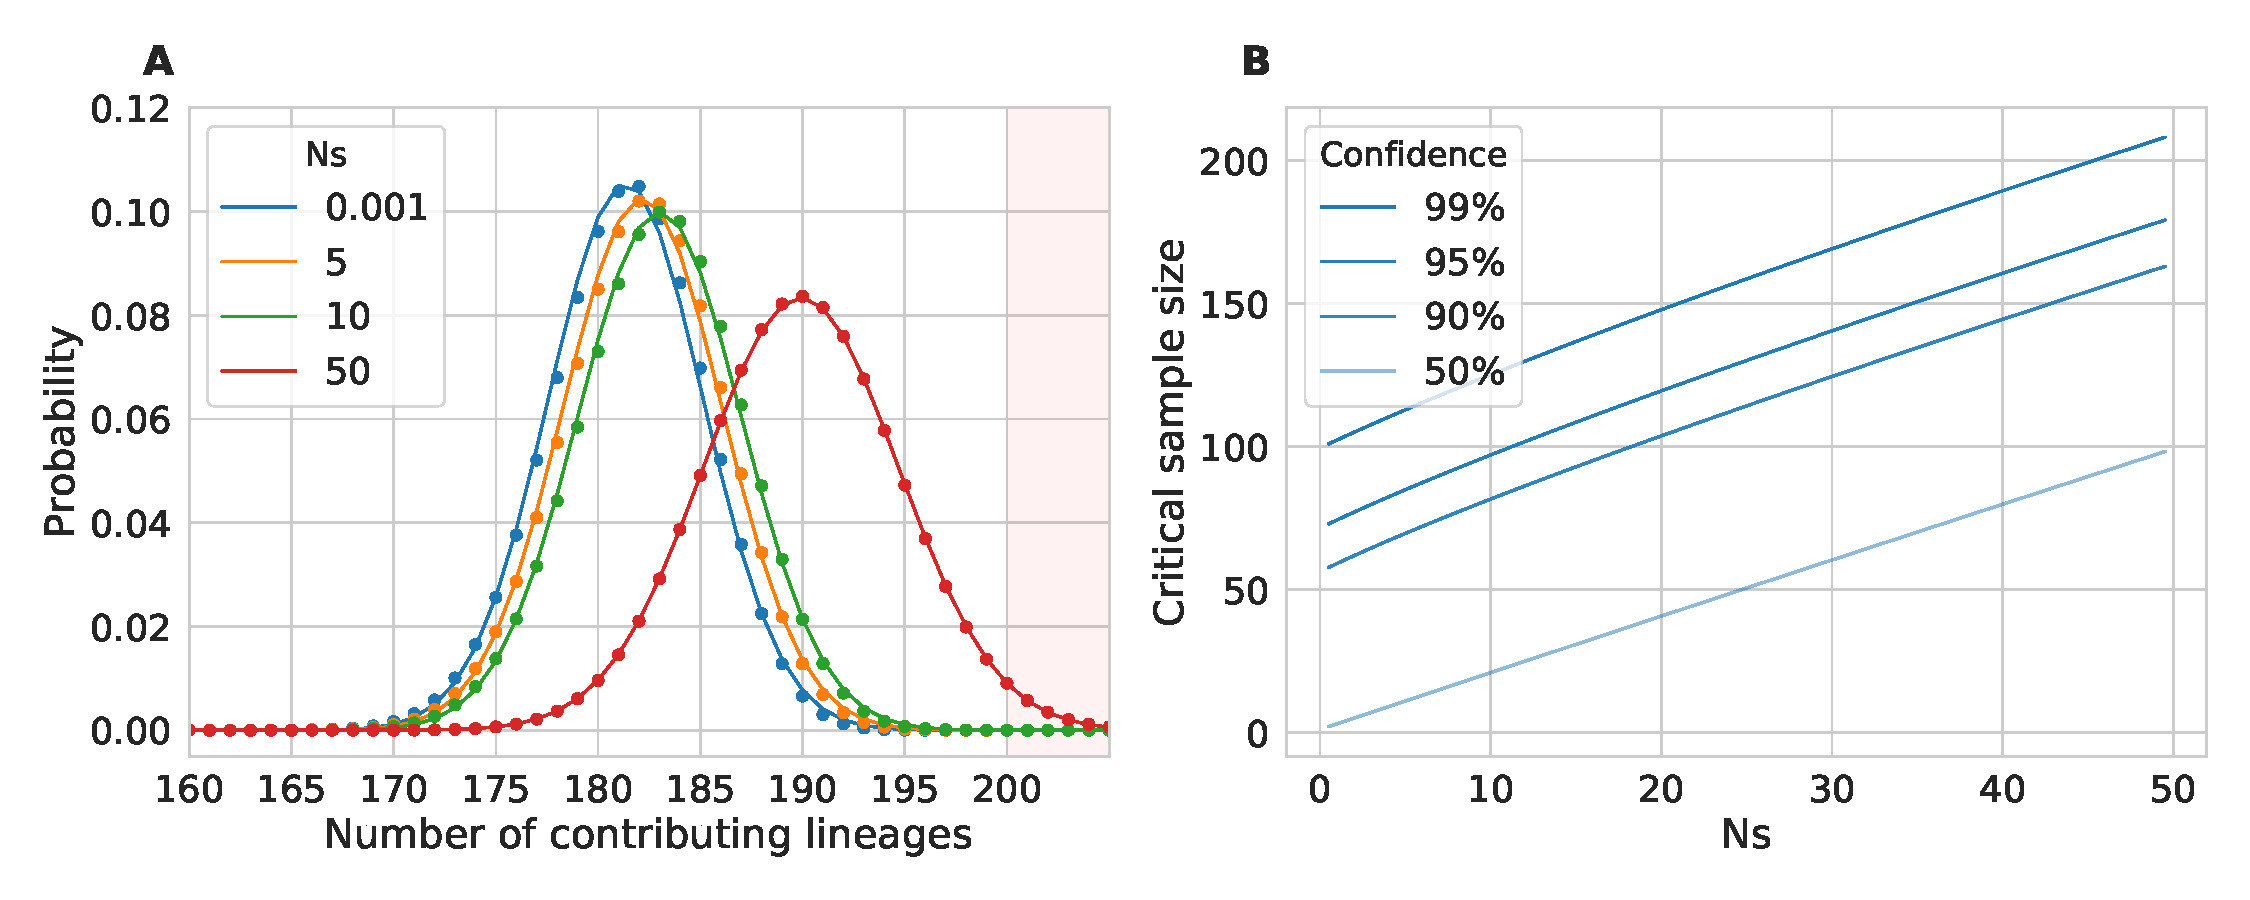
\includegraphics[width=\textwidth]{fig/combined.pdf}
  \caption{\textbf{A} The distribution of number of required lineages with $n_0=200$, $x_p=1$. Shaded
    red area shows missing probability, where $n_p > n_o$. Points represent the exact probability one
    generation into the past (Eq. \ref{eq:lineages-in-past}), solid lines - Gaussian approximation
    (Eq. \ref{eq:gaussian}). \textbf{B} Sample size ($n_o$) as a fraction of population size ($N$)
    such that we have $99\%$ confidence that no lineages are missing, derived from the Gaussian
    approximation. The dotted line indicates regimes where the Gaussian approximation is likely inaccurate. 
     In both panels, $N=1000$.}
  \label{fig:combined}
\end{figure}

The distribution in Eq. \ref{eq:lineages-in-past} can quickly be calculated numerically, but
provides little intuition. To get more intuition, we will compute the
expectation and variance of this distribution, and show that it can be accurately approximated by a
Gaussian distribution in useful parameter regimes.

\section{Asymptotic closure properties}
\label{sec:asympt}


Using the law of total expectation, we can write the expectation $E[n_p-n_o | n_o]$ as 
\begin{equation*}
  \begin{aligned}
    \label{eq:lineages-approx}
    E[n_p-n_o | n_o] &=        E[n_p | n_o]       - n_o \\
                     &=E_{n_g} E_{n_p}[n_p | n_g] - n_o.
  \end{aligned}
\end{equation*}
Assuming $x_p=1$, the expectation over $n_p$ is simply that of the occupancy distribution \cite{Wakeley2009}.

\begin{equation*}
  \begin{aligned}
    \label{eq:lineages-derive}
    \hat{E}[n_p -n_o | n_o]
    & =   E_{n_g}\left[N\left[1-\left(1 - \frac{1}{N} \right)^{n_g} \right]\right]- n_o\\
    & =   N-N  E_{n_g}\left[\left(1 - \frac{1}{N} \right)^{n_g} \right] -n_o. 
  \end{aligned}
\end{equation*}

As mentioned above, the number of selective deaths, $n_g-n_o$ follows a negative binomial
distribution. We can use the moment generating function of the negative binomial to compute the
expectation of $k^{n_g}$ for any constant $k$:

\begin{equation}
E_{n_g}[k^{n_g}] = k^{n_o}  \left(\frac{1-s}{1-sk}\right)^{n_o}.
\label{eq:identity}
\end{equation} 
Thus we can write 
\begin{align}
  \label{eq:gauss-mean}
  \hat{E}[n_p -n_o | n_o] &= N-N\left( 1 - \frac{1}{N} \right)^{n_o}\left( \frac{1-s}{1-s \left( 1 - \frac{1}{N} \right)}\right)^{n_o}-n_o.
\end{align}
Taking the terms of order up to $\frac{1}{N}$ gives

\begin{equation*}
    \label{eq:lineages-approx}
    \hat{E}[n_p-n_o | n_o] \approx n_os - \frac{n_o (n_o-1) }{2N}. 
\end{equation*}

We thus have the usual interplay of selection and drift. Solving for $ \hat{E}[n_p -n_o | n_o]<0$
yields, to leading order,

\begin{equation}
  \label{eq:critical-sample}
  n_o^* \ge 2Ns.
\end{equation}

This represents a critical sample size (Fig.
\ref{fig:apx:critical-normal}) where there is more drift than selection events, on average. 
(If we want to include the derived allele frequency in the parental generation,
\eqref{eq:critical-sample} becomes $2Nsx_p$, or $4Nsx_p$ in a diploid model). %However, closure of
%the recursions requires not only that drift occurs more often than selection on average, but almost
%always.

To ensure closure of the recursions, our next step is to compute the variance of this distribution, $\operatorname{Var}[n_p-n_o | n_o].$ The detailed
calculations using the moment generating function and the exact result are provided in the Appendix. To leading order in $s,$ $n_o/N,$ and $1/N,$ the variance is 


\begin{equation}
  \begin{aligned}
    \operatorname{Var}[n_p-n_o | n_o] &\simeq
   N(  \frac{n_o}{N} s + n_o (n_o-1)^2/(2 N^2)) = n_o s +   n_o (n_o-1)^2/(2 N).
    \label{eq:gauss-var}
  \end{aligned}
\end{equation}

Thus the mean and variance to leading order are those of the Skellam distribution: the increase in lineages can be modelled, to lowest order, as the number of lineages 
gained through selection (modelled as Poisson with mean  $ n_o (n_o-1)^2/(2 N)$) minus the number of lineages lost to drift (modelled as Poisson 
with mean  $ n_o (n_o-1)^2/(2 N)$). As the number of drift and selection events get larger,
the Skellam distribution can be approximated as a Gaussian.

\begin{equation}
  P(n_p|n_o) \sim \mathcal{N}(\mu, \sigma)
  \label{eq:gaussian}
\end{equation}

Figure \ref{fig:combined}A shows the excellent agreement between the exact distribution and the Gaussian approximation 
(using the exact variance from Equation \eqref{eq:exact-var}.
%\sgcomment{I thought that we had citations here that showed why the gaussian approximation made sense?}
By contrast, we don't expect this approximation to work well if the sample size is so small that few 
drift events occur at a given generation, (say,  $\frac{{n_o}^2}{2N} < 10$).
 
Under the Gaussian approximation, we can numerically compute the quantiles of the Gaussian distribution to find a sample size
where we are, for example, $99\%$ confident that there will be no missing lineages --- i.e.,  $P(n_p -n_o >0) < 0.01$. 
\sgcomment{It would be worth explaining why/whether this is a reasonable criterion. 
Would this mean that we are loosing 1\% of probability at each generation? That sounds pretty bad.
 }


The Gaussian approximation using leading order terms provides intuition about regimes where we expect drift to 
almost always overtake selection. 
Concretely, if we solve for the sample size $n_z$ required such that the ratio of the mean to the standard deviation is $z$,
we get, for $n_z>>1$,
 \begin{equation}
 n_z \leq 2 \sqrt{N} z + 2N x s.
\label{eq:nz}
\end{equation}
 \sgcomment{There is an approximation here -- put derivation in appendix}
The second term is just the condition that there are more coalescence events than selection events, on average. The first term is independent of $s$ and 
can be interpreted as a condition that there are sufficient drift events per generation to ensure that the probability 
of having zero drift event is weak: $n_z = 2 \sqrt N z$ implies $\frac{n^2}{2N}= 2 z.$ One interpretation is that 
we need at least a few expected coalescence events per generation to ensure that every selective event is 
compensated by a coalescence event. 

 \sgcomment{
Figure  \ref{fig:combined}B shows a comparison of leading-order terms to computations using the exact
expressions for the mean and variance.}

%Figure \ref{fig:combined}B shows the ratio of sample size to population size ($n_o/N_e$), for the $99\%$  
%confidence for different values of $N.$ The dashed lines indicate where the Gaussian approximation may be
%invalid: $\lambda < 10$.

Equation \eqref{eq:nz} and Figure  \ref{fig:combined}B show that the truncation can be accurate even for strong selection 
and sample sizes much smaller than the full population size. 


%The required sample size as a function 
%of the desired confidence is shown on Figure \ref{fig:apx:critical-normal}.
%For smaller sample size, the exact distribution \eqref{eq:lineages-in-past} can be used.

\subsection{Integrating over several generations} 

If the sample size is large enough that $E[n_p-n_o]<0$, but not large enough that
$P(n_p>n_o) \ll 1,$ we can improve the truncation by integrating over more than one generation.
Lineages gained by selective death at one generation can be compensated for by genetic drift at
another generation.
If we restrict our attention to a small number $g$ of generations, we approximate the change 
in the number of lineages as we go back in time as a random walk with constant mean and 
variance. In this case, both the mean and variance will be scaled by a factor $g$ relative 
to the single-generation case, and Equation \eqref{eq:nz} becomes 
\begin{equation}
 n_z \lessapprox 2 z\sqrt{N/g} + 2N x s.
\label{eq:nz}
\end{equation}
 

Thus we expect to find asymptotic closure for $n_o> 2Ns$ given enough generations. 
 

% Informally, the expected change $E[n_g-n_o]$ in the number $n_g$ of lineages in
%the grandparent generation relative to $n_o,$ and the variance $\operatorname{Var}[n_g-n_o]$ will be
%roughly double those over a single generation. Thus the $z$-score determining the amount of
%unnaccounted-for lineages in the normal approximation,
%$z= E[n_g-n_o] / \sqrt{\operatorname{Var}(n_g-n_o)}$ will increase roughly by a factor $\sqrt{2}$.


Such multi-generation transition matrices can also be computed iteratively. If $n_{p'}$ is the number of sampled
lineages in the grandparental generation, and $i_{p'}$ is the number of derived alleles among those,
and we define $P(i_o, \mathcal{S'}_{n_{p'}} | \mathcal{C}'(i_{p'}, n_{p'}))$, as above, as the probability of
drawing $i$ derived alleles and  the event $\mathcal{S'}_{n_{p'}}$ that we are using exactly $n_{p'}$ grandparental alleles given the event
$\mathcal{C'}(i_{p'}, n_{p'})$ that $i_{p'}$ of the first $n_{p'}$ grandparental alleles are
derived, we can condition on the number of contributing parental alleles $n_p$ and the number of
derived alleles $i_p$ among them in the parental generation:

\begin{equation}
  \begin{split}
    P(i_o, \mathcal{S}'_{n_{p'}} | \mathcal{C}'(i_{p'}, n_{p'})) & = \sum_{i_p,n_p} P(i_o, \mathcal{S}'_{n_{p'}} ; \mathcal{C}(i_p,n_p), \mathcal{S}_{n_p} | \mathcal{C}'(i_{p'}, n_{p'}))\\
    &= \sum_{i_p,n_p}  P(i_o, \mathcal{S}_{n_{p}} | \mathcal{C}(i_p,n_p), \mathcal{S'}_{n_p'} ; \mathcal{C}'(i_{p'}, n_{p'})) P(\mathcal{C}(i_p,n_p), \mathcal{S'}_{n_{p'}} | \mathcal{C}'(i_{p'}, n_{p'})) \\
    &=  \sum_{i_p,n_p}  P(i_o, \mathcal{S}_{n_{p}} | \mathcal{C}(i_p,n_p))) P(\mathcal{C}(i_p,n_p), \mathcal{S'}_{n_{p'}} | \mathcal{C}'(i_{p'}, n_{p'})) \\
    &=   \sum_{n_p}^{n_{p,max}} T_{n_p,n_o} T_{n_{p'}, n_p},
  \end{split}
\end{equation}
where the sum over $i_p$ is part of the product of the transition matrices $T$. Since each matrix
product takes $O(n_o n_p n_{p'})$, and there are at most $O(n_{p,max})$ such products, the computation of this
matrix product takes at most $O(n_o n_{p,max}^2 n_{p'}).$ We expect that this scaling can be improved upon in numerical 
implementations by summing over values of $n_p$ that contribute appreciably. 
In addition, we need to build the matrices $T_{n_p', n_p}$. 
In the recursive approach, the computation of the matrix for the largest sample includes the computation of matrices for
smaller sample sizes, so the computation time is at most $O(r_{max} n_{p,max}^2, n_{p',max}^2).$ 
If we construct a truncated matrix, $n_{p',max} =n_o$, and we find  $O(r_{max} n_{p,max}^2, n_{o}^2).$
In the exact formulation, $n_p$ can be as large as $ r_{max} n_o,$ however in numerical application 
with $s< 0.5$ we expect that using a cutoff with $n_{p,max}= 2 n_o$ would provide excellent convergence, 
hence an overall scaling of   $O(r_{max} n_{o}^4)$ for the construction of the matrices and $O(n_o^4)$ for the matrix product.
Thus a naive construction of a transition matrix over $g$ generations would require  $O( (t + r_{max} ) n_o^4).$



\section{Conclusion}
\label{sec:conclusion}
\sgcomment{This conclusion needs some work.}

%Classically, the coalescent considers models in the absence of natural selection. Since selection
%can increase the number of contributing lineages back in time, the coalescent can no longer be
%represented by trees, but instead acquires a graph structure. The ancestral selection graphs
%\citep{KroneNeuhauser1997} deal with this in the limit of large population size ($N$).

The large population size approximation implies that the sample size $n$ is much smaller than the
whole population ($n \ll N$), so it is unlikely that more than one coalescent event will happen per
generation. However, recent work \citep{BhaskarEtAl2014,NelsonEtAl2019} pointed out that this
assumption is unreasonable with sample sizes pertinent to modern experiments. As a result, models
that consider multiple coalescent events per generation are gaining increased relevance in the field
.
In this work we show that increasing the sample size has another unexpected consequence. As sample
size increases, the larger number of lineages needed due to selection can be masked by coalescent
events. In this sense, the large sample size rescues the model from effects of selection. This means
that recursion equations needed to calculate sample properties are asymptotically closed with large
population size.

At first approximation, $n_o^*=2Nsx_p$ is a critical sample size, where the decrease of lineages due to
coalescent back in time out-competes the increase due to selection (eq. \ref{eq:critical-sample}).
Further, we derive the full probability distribution for the number lineages needed with given
selection coefficient and sample size (Eq. \ref{eq:lineages-in-past}). Unfortunately, the
distribution does not have a closed form, so we derive a normal approximation to the number of
lineages that contribute to a sample (Eq. \ref{eq:gaussian}). The normal approximation
then allows us to get a quantile function that we use to find if the model preserves closure with
some confidence level.

This work has several implications. First, we can combine the model described here with the
jackknife approximation \citep{JouganousEtAl2017}. This will allow us to construct a more robust
inference framework that can account for large sample size and strong selection.

Further, the results here suggest that effect of weak selection may be detectable in studies with
large sample sizes. This may open up a way for new investigations of natural selection in population
genetics.

\bibliography{disco}

\section{Appendix}
\renewcommand{\thefigure}{S\arabic{figure}}
\setcounter{figure}{0}

\subsection{Missing lineages}

\begin{figure}
  \centering
  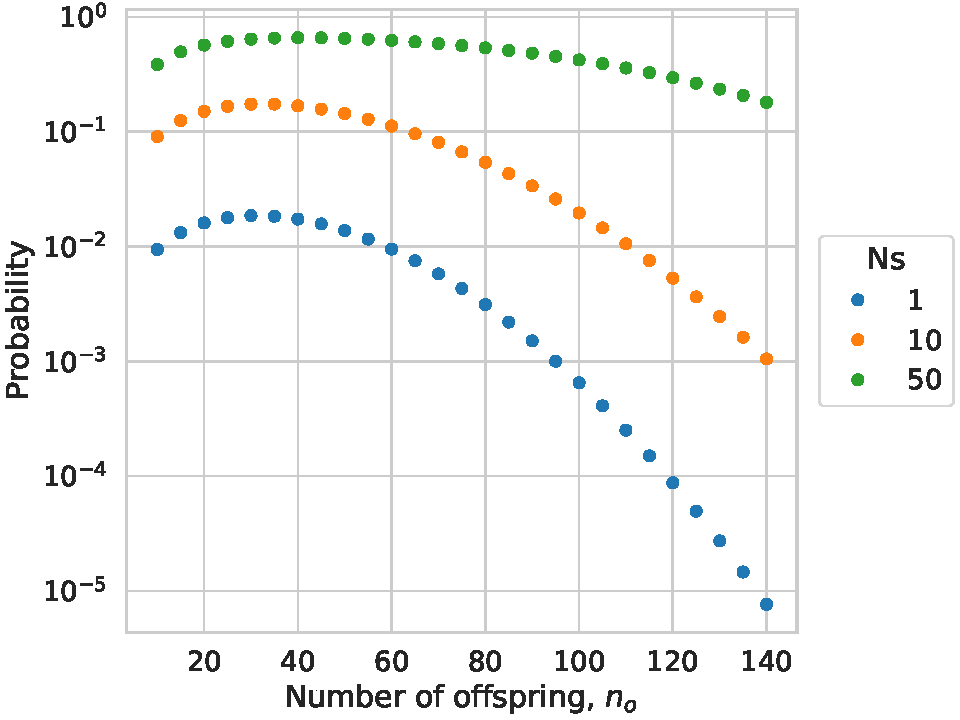
\includegraphics[width=\textwidth]{fig/missing.pdf}
  \caption{Probability that there are more contributing parents than offspring, $n_p > n_o$.
    Calculated as $1-\sum_{i_o} \mathbf{Q}_{n_o}{i_p, i_o}$, $N=1000$.}
  \label{fig:apx:missing}
\end{figure}

\subsection{Quantiles of the Gaussian approximation}

Figure \ref{fig:apx:critical-normal} shows the critical sample size for a given quantile of the normal
approximation, as a function of the population-scaled selection coefficient. The $50^{\text{th}}$
percentile corresponds to the mean calculated in equation \ref{eq:critical-sample} ($\approx 2Ns$).
If we want to ascertain that the distribution is closed with increased confidence, we require a
larger number of lineages. All curves assume $N=1000$.

\begin{figure}
  \centering
  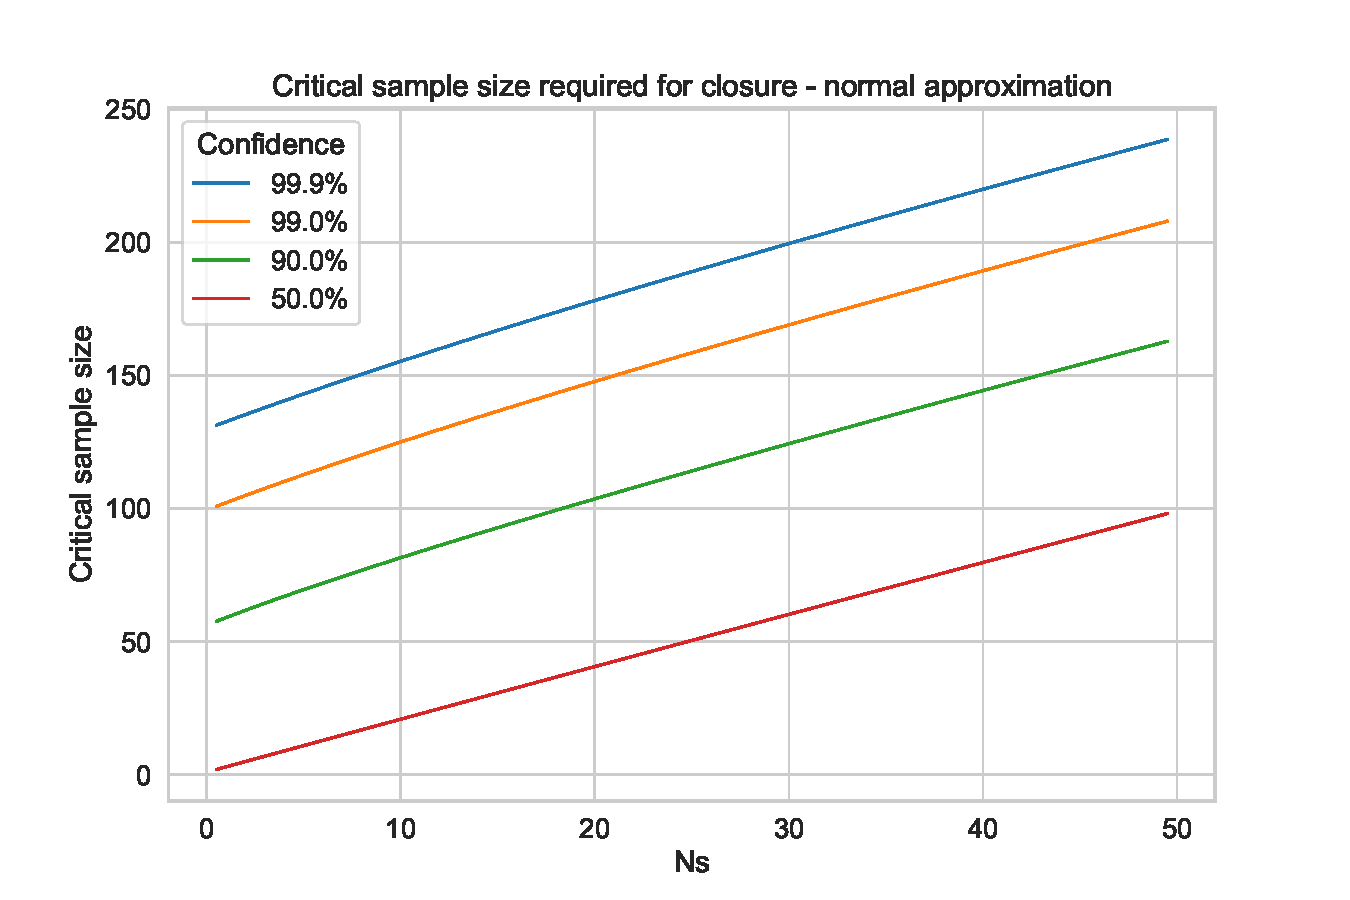
\includegraphics[width=\textwidth]{fig/critical_normal.pdf}
  \caption{Critical sample size that is required for a given closure confidence level. The
    $50^\text{th}$ percentile corresponds to the mean in the equation \eqref{eq:critical-sample}. Note that the
    normal approximation is invalid for $Ns=0$, where the occupancy distribution should be used. All
    lines are calculated with $N_e=1000$.}
  \label{fig:apx:critical-normal}
\end{figure}

\subsection{Variance of number of contributing lineages}
\label{subsec:apx:variance}

We can obtain the variance of the distribution $P(n_p | n_o)$ by using the law of total variance:

\begin{equation}
  \label{eq:apx:var}
\Var\left[n_p-n_o \right] = \Var_{n_g}\left[E\left[n_p-n_o | n_g \right]\right]+  E_{n_g}\left[Var\left[n_p-n_o | n_g \right]\right] 
\end{equation}

The expectation in the first term can be derived from the occupancy distribution and the identity
\ref{eq:identity}:

\begin{equation}
\begin{split}
\Var_{n_g}\left[E\left[n_p-n_o | n_g \right]\right] &= \Var_{n_g}\left[E\left[n_p| n_g \right]\right] \\
&= \Var_{n_g}\left[N\left(1-(1-\frac{1}{N})^{n_g} \right) \right] \\ 
&= N^2 \Var_{n_g}\left[(1-\frac{1}{N})^{n_g} \right] \\
&= N^2 \left( E_{n_g}\left[(1-\frac{1}{N})^{2n_g} \right] - E_{n_g}\left[(1-\frac{1}{N})^{n_g} \right]^2\right) \\
&= N^2 \left( \left(1-\frac{1}{N}\right)^{2n_o} \left(\frac{1-s}{1-s  \left(1-\frac{1}{N}\right)^2}\right)^{n_o} 
-   \left(1-\frac{1}{N}\right)^{2n_o} \left(\frac{1-s}{1-s  \left(1-\frac{1}{N}\right)}\right)^{2n_o} \right) \\
\end{split}
\end{equation}

The variance of the second term is the variance of the occupancy distribution \cite{}:

\begin{equation}
\begin{split}
E_{n_g}\left[Var\left[n_p-n_o | n_g \right]\right] & = E_{n_g}\left[N ((N - 1) (1 - 2/N)^{n_g} + (1 - 1/N)^{n_g} - N (1 - 1/N)^{2 n_g}) \right] \\
& = N (N-1)  \left(1-\frac{2}{N}\right)^{n_o} \left(\frac{1-s}{1-s  \left(1-\frac{2}{N}\right)}\right)^{n_o} +  \left(1-\frac{1}{N}\right)^{n_o} \left(\frac{1-s}{1-s  \left(1-\frac{1}{N}\right)}\right)^{n_o} \\
&-N  \left(1-\frac{1}{N}\right)^{2n_o} \left(\frac{1-s}{1-s  \left(1-\frac{1}{N}\right)^2}\right)^{n_o}. 
\end{split}
\end{equation}

The two terms can be summed together to provide an analytical expression for the variance of $n_p$, and we get


\newcommand{\vara}[1]{\left(1-\frac{#1}{N}\right)}
\newcommand{\varb}[1]{\left(\frac{1-s}{1-s #1}\right)}

\begin{equation}
  \begin{aligned}
    \operatorname{Var}[n_p-n_o | n_o] &=
    N^2\left( \vara{1}^{2n_o}\varb{\vara{1}^2}^{n_o}-\vara{1}^{2n_o}\varb{\vara{1}}^{2n_o} \right) + \\
    &+ N(N-1)\vara{2}^{n_o}\varb{\vara{2}} + \vara{1}^{n_o}\varb{\vara{1}}^{n_o} - \\
    &- N\vara{1}^{2n_o} \varb{\vara{1}^{2}}^{n_o}.
    \label{eq:exact-var}
  \end{aligned}
\end{equation}



\subsection{Selection case}
\label{subsec:apx:tpm}

\ikcomment{I've changed the event $r$ to $c$ in the main text (to avoid the unlikely confusing for
  $r$, the number of failures). This will need to be propagated in here, too}.

Due to selective deaths, the number of lineages ($n_p$) that contribute to the current generation
can be larger than the number of offspring ($n_o$), and especially so with strong selection. Because
the number of sampling configurations can be large, we use dynamic programming to estimate
$\mathbf{P}_{n_p,n_o}$ by summing over the possibilities for the last successful draw. Using the
probability interpretation of the transition matrix,
$\mathbf{P}_{n_p,n_o}(i,j) = P(i, n_p | r(j, n_p)),$ the probability that we draw $i$ derived
offspring and exactly $n_p$ parental offspring given that $j$ of the first $n_p$ sampled parental
alleles are derived. The last successful draw event can be specified by the number
$t \in \{0,\infty\}$ of prior failed draws due to selection since the last successful draw, the
allele $a \in {A, D}$ selected, and the event $c$ of whether or not the sampled parental allele was
previously drawn $c\in \{True, False\}$. We also consider the event $s \in \{True, False\}$ of
whether the last draw was successful. Finally, let us define the event $E_{n_o,t}(i,n_p)$ that we
have drawn $i$ derived offspring among $n_o$ successful draws followed by $t$ failures, and that
this required exactly $n_p$ parental lineages.

\begin{equation}
\begin{split}
P(i, n_p | r(j, n_p)) = P(E_{n_0,0}(i,n_p)  | r(j, n_p)) &=  \sum_{a, c,t} P(a,c,t; E_{n_o,0}(i,n_p)  | r(j, n_p)) 
 \end{split}
\end{equation}

Let us consider the term $a=A$, $c=False$ \sgcomment{We could use a better notation here, eg using
  tikz. }

\begin{equation}
  \begin{split}
    P(a=A,c=False,t; E_{n_o,0}(i,n_p)  | r(j, n_p)) &= P(a=A, c=False, t,s=True; E_{n_o,t}(i,n_p-1) | r(j, n_p))\\
    &= P(a=A, c=False, t; E_{n_o,t}(i,n_p-1) | r(j, n_p))\\
    &=P(a=A, c=False, t ; E_{n_o,t}(i,n_p-1); r(j, n_p-1) | r(j, n_p))\\
    &=P(a=A, c=False, t ; E_{n_o,t}(i,n_p-1)| r(j, n_p-1)  r(j, n_p)) P(r(j, n_p-1) |  r(j, n_p))\\
    &=P(c=False, t;  E_{n_o,t}(i,n_p-1) | r(j, n_p-1)  r(j, n_p)) \frac{n_p-j}{n_p}\\
    &=P(c=False | t;  E_{n_o,t}(i,n_p-1) | r(j, n_p-1)  r(j, n_p)) P(t;  E_{n_o,t}(i,n_p-1) | r(j, n_p-1)  r(j, n_p)) \frac{n_p-j}{n_p}\\
    &=\left(1-\frac{n_p-1}{N}\right) P(t;  E_{n_o,t}(i,n_p-1) | r(j, n_p-1)  r(j, n_p)) \frac{n_p-j}{n_p}\\
    &=\left(1-\frac{n_p-1}{N}\right) P(t;  E_{n_o,t}(i,n_p-1) | r(j, n_p-1)) \frac{n_p-j}{n_p}
  \end{split}
\end{equation}

where the fourth line uses Bayes rule, and most other lines are exercises in rewriting the same
event in different ways. Other combinations of $a$ and $c$ also yield expressions in terms of
probabilities $P(t; E_{n_o,t}(i,n_p) | r(j, n_p))$ for the state prior to the successful draw
\sgcomment{write down final results?}.


These can be similarly expressed as recursions over the last draw. Selection only affects derived alleles, but it can occur after both coalescence and non-coalescence events. 
\begin{equation}
\begin{split}
P(t;  E_{n_o,t}(i,n_p) | r(j, n_p)) = \sum_c P(c, t;  E_{n_o,t}(i,n_p) | r(j, n_p)).
\end{split}
\end{equation}

For example, the $c = True$ term can be written as 
 \begin{equation}
\begin{split}
P(c=True, t;  E_{n_o,t}(i,n_p) | r(j, n_p)) &= P(c=True, a=D, s=False, t;  E_{n_o,t}(i,n_p) | r(j, n_p))\\
&= s P(c=True, a=D, t;  E_{n_o,t-1}(i-1,n_p) | r(j, n_p))\\
&= s \frac{j}{N} P( t;  E_{n_o,t-1}(i-1,n_p) | r(j, n_p)),\\
\end{split}
\end{equation}

\sgcomment{I think this might want to be: }
 \begin{equation}
\begin{split}
P(c=True, t;  E_{n_o,t}(i,n_p) | r(j, n_p)) &= P(c=True, a=D, s=False, t;  E_{n_o,t}(i,n_p) | r(j, n_p))\\
&= s P(c=True, a=D, t;  E_{n_o,t-1}(i,n_p) | r(j, n_p))\\
&= s \frac{j}{N} P( t;  E_{n_o,t-1}(i,n_p) | r(j, n_p)),\\
\end{split}
\end{equation}

and similarly for $c=False$ \sgcomment{Write out? TODO, not complete}.  

 \begin{equation}
\begin{split}
P(c=False, t;  E_{n_o,t}(i,n_p) | r(j, n_p)) &= P(c=False, a=D, s=False, t;  E_{n_o,t}(i,n_p) | r(j, n_p))\\
&= s P(c=False, a=D, t;  E_{n_o,t-1}(i,n_p-1) | r(j, n_p))\\
&= s \frac{j}{N} P( t;  E_{n_o,t-1}(i,n_p) | r(j, n_p)),\\
\end{split}
\end{equation}


Putting this all together \sgcomment{pseudocode?}, we can perform an iteration over all $n_o.$ For
each $n_o,$ we will compute all terms of the form $P(E_{n_0,0}(i,n_p) | r(j, n_p)),$ for
$i\in\{0,\ldots,n_0\}$, $j\in \{0,\ldots,n_p\}$, and $n_p \in\{1,\ldots,n_{p,max}\}.$ We further
need to iterate over the possible number of failed selective events. If we only allow a maximum
amount of failed selected events of $t_max$ for each successful draw, the number of terms we must
compute is of order $t_max n_p^4$. The number of computations for each term is constant and only
depends on previously computed terms.

To ensure that probabilities do sum to one despite the $t_max$ cutoff, we modify the Wright-Fisher model by imposing a successful draw after $t_max-1$ attempt. Thus terms

$P(a=D,c,t_{max}; E_{n_o,0}(i,n_p)  | r(j, n_p))$ will lose a factor $(1-s)$.   



\end{document}
